\chapter{Analýza a implementace serverové části}\label{ch:server}

\chaptersummary{
   \begin{ul}
      \item popis architektury serverové aplikace a metod zvolených pro realizaci,
      \item volba úložiště zdrojových kódů,
      \item rozbor komplexnějších funkcionalit a aspektů realizace.
   \end{ul}
}

Implementace serverové části na základě zadání a definované specifikace \g{IS} spočívá v anaýze aktuální monolitické architektury (z předchozí práce) a její přespis do architektury mikroslužeb s využitím zkušeností získaných a popsaných v kapitolách~\enquote{\nameref{ch:msa-intro}} a~\enquote{\nameref{ch:msa-data}}.

Ačkoliv původní implementace měla vyřešeno dost aspektů z hlediska funkcionality, přechod na novou architekturu způsobem využití exitujícíh zdrojových kódů by odhadem zabral víc času, než nová realizace s pouhou inspirací z původního systému.
Z tohoto důvodu bylo rozhodnuto napsat nový základ pro mikroslužby, který by víc vyhovoval aktuálním potřebám.
Pro novou relizaci bylo rovněž vybráno jiné \g{ORM}, které přineslo zjednodušení během vývoje za cenu změny implementace většiny funkcionalit spojených s relační databází, zejména funkcionalitou migrací.
Detailní popis změn a přínosů je uveden v následujících podkapitolách.

\newpage



\section{Architektura}\label{sec:server-arch}

Základním krokem pro návrh architektury serverové části se stal výběr typu dekompozice poskytnuté specifikace.
v rámci požadavků na možnou výměnu zdroje s projekty, nebo i budoucí přechod na jiný způsob autorizace, se zdala nejvhodnější dekompozice dle subdomén.

Dekompozice se provedla na následující mikroslužby:

\begin{ul}
   \item \textbf{ms-users} – uživatelská data a vše, co je potřeba pro správu uživatelů.
   \item \textbf{ms-auth} – autentizační funkcionalita, kontrola validity autorizačních údajů a přístupových práv.
   \item \textbf{ms-projects} – služba pro správu projektových dat.
   Ukládá v relační databázi metadata o projektech a deleguje úpravy obsahů na vnější git úložiště.
   \item \textbf{ms-interpreters} – správa registovaných interpretů a jejich verzí.
   \item \textbf{ms-communication} – zpracovávání komunikačních zpráv s uživateli, jako jsou e-maily a upozornění.
   \item \textbf{ms-monitoring} – služba pro centrální kontrolování stavů mikroslužeb a logování zpráv.
\end{ul}

K tomu v rámci architektury byly přidány následující služby:

\begin{ul}
   \item \textbf{API Gateway} – implementace API Gateway fasády s pomocí nginx, která předává komunikaci klienta patřičným mikroslužbám.
   \item \textbf{SQL databáze} – \g{SQL} databáze v podobě PostgreSQL pro správu relačních dat.
   \item \textbf{NoSQL databáze} – NoSQL databáze v podobě MongoDB pro správu logovacích dat.
   \item \textbf{Message Broker} – RabbitMQ broker pro asynchronní komunikační kanály mezi mikroslužbami.
\end{ul}

Komunikace všech těchto je znázorněna a obrázcích~\ref{fig:server-arch} a~\ref{fig:server-github}.

\begin{figure}[htbp]
   \centering
   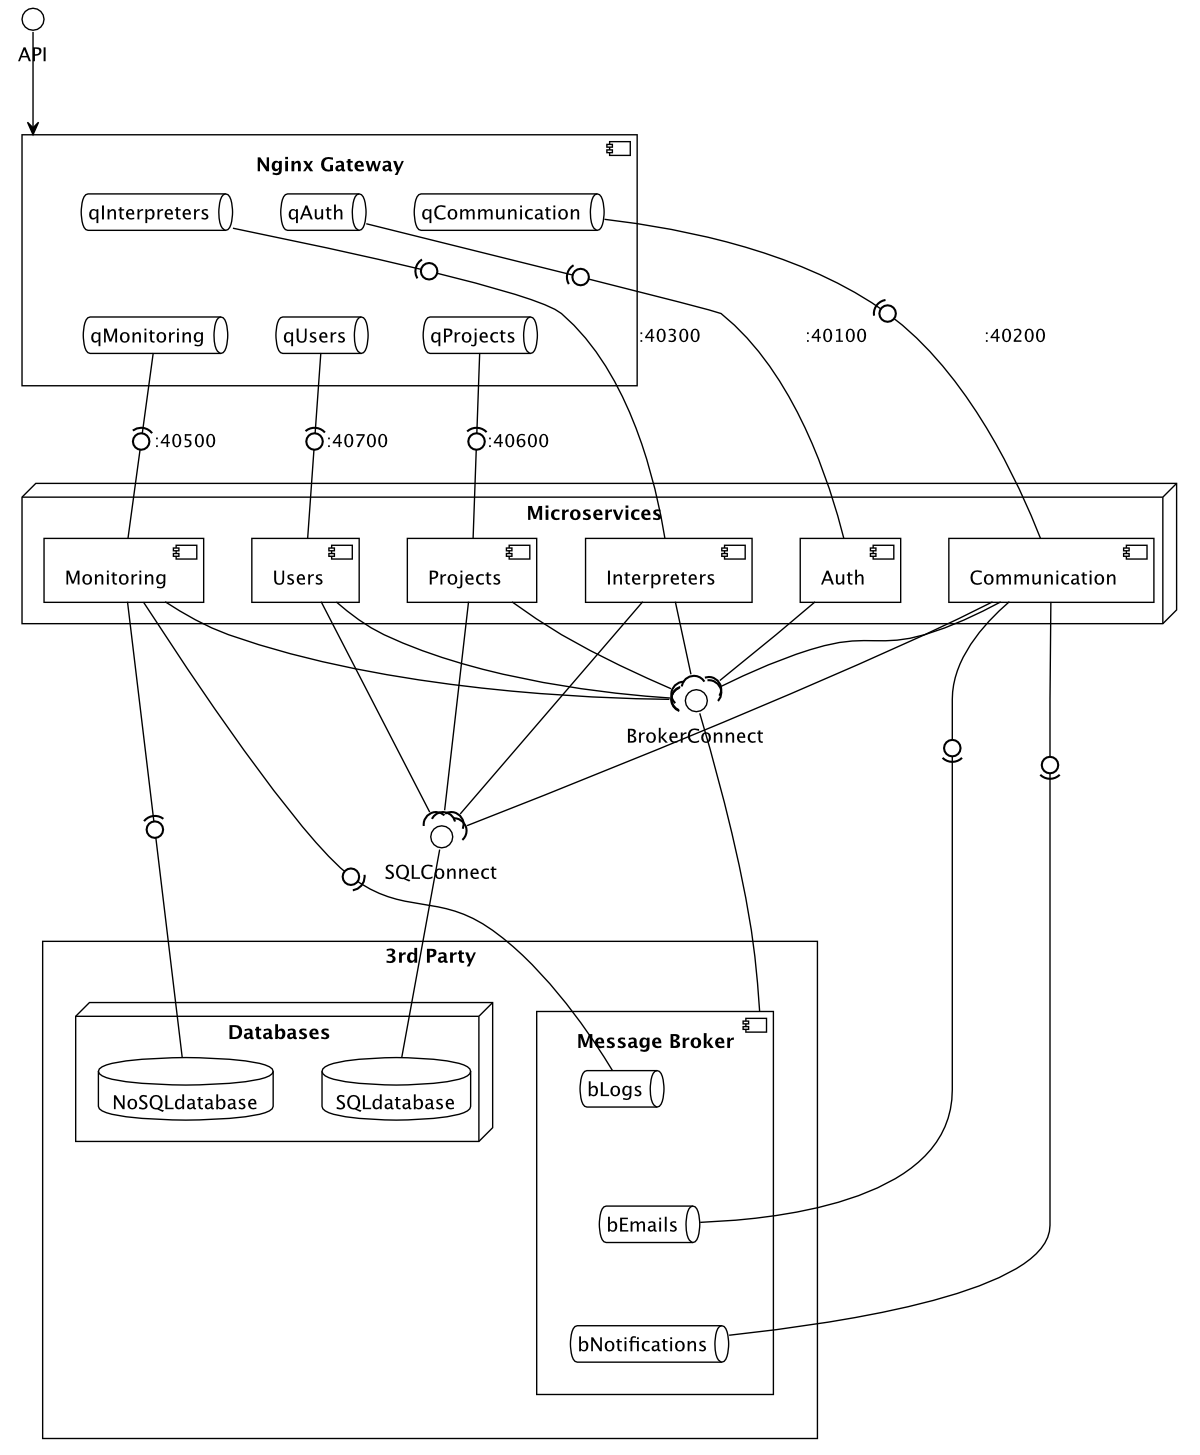
\includegraphics[max width=\textwidth]{assets/arch-be}
   \caption{Architektura serveru}\label{fig:server-arch}
\end{figure}

\begin{figure}[htbp]
   \centering
   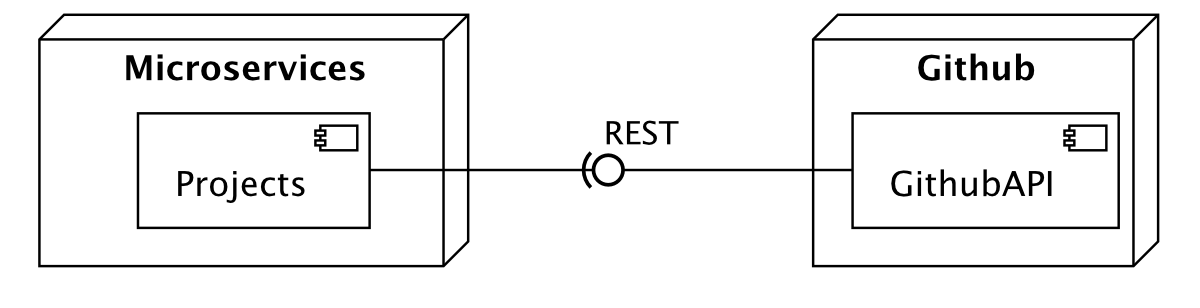
\includegraphics[max width=\textwidth]{assets/arch-github}
   \caption{Vazba mikroslužby na Github}\label{fig:server-github}
\end{figure}

Gateway v této implementaci rozděluje veškerou komunikaci se serverem na několik nginx streamů, které se rozpoznávají dle unikátních \g{URI} prefixů.
Každý stream komunikuje právě s jednou mikroslužbou na vlastním portu (viz obrázek~\ref{fig:server-arch}).
Mikroslužby jako takové jsou organizovány choreografickým způsobem a mohou volně volat rozhraní jiných mikroslužeb v rámci sítě.
Pro danou komunikaci byl zvolen typ synchronní komunikace přes \g{REST} rozhraní, jako nejméně náročný pro implementaci.
Výjimku však tvoří speciální případy, které vyžadují jistotu doručení zprávy, jedná se o logování, odesílání e-mailů a odesílání důležitých notifikací konkrténím účtům.
V těchto případech je použit broker zpráv, který funguje jako pojistka, že se zpráva neztratí v případě přetížené nebo nedostupné mikrošlužby.
Funguje na principu producent-konzument, tzn.
jakmile se objevuje služba, která uložené zprávy může zpracovávat, tak ji jsou předány.
V aktuální implementaci takové role zastupují mikroslužby \h{Communication}, která odbavuje e-maily a upozornění, a \h{Monitoring}, jenž se stará o logování.

Z hlediska úložišť některé mikroslužby jsou napojené na \g{SQL} a NoSQL databáze, speciální případ tvoří však mikroslužba \h{Projects}, která vyžaduje existenci Github organizace s přístupovými právy pro správu repozitářů, aby v nich mohla uchovávat existující uživatelské projekty (viz kapitola~\enquote{\nameref{subsec:server-db-github}}).



\section{Struktura repozitářů}\label{sec:repository-structure}

V rámci volby způsobu uspořádání repozitářů byl vybrán kombinovaný způsob popsaný v kapitole \enquote{\nameref{subsec:msa-deployment-code}}.
Každá mikrozlužba získala vlastní repozitář, jenž by mohl být vyvíjen naprosto separovaně.
Zároven se ale vytvořil repozitář, který definoval všechny mikroslužby jako git submoduly a přidal k tomu samostatně složku s Gateway, skripty pro rychlou tvorbu potřebných \h{.env} konfigurací ve všech mikroslužbách a \h{docker-compose} soubory pro vývojové a produkční prostředí.

Takoté řešení poskytlo možnost instantně získávat téměř hotové (až na konfigurace) prostředí, navíc s variantou odděleného spuštění persistentních prvků (typu databází).
Věškerý vývoj \g{IS} pak probíhal způsobem, že na externím serveru byly spuštěné databáze, Gateway a broker, které se mohly připojit k lokálnímu stroji pro vývoj, který by zatížen pouze potřebnými prvky - mikroslužbami a klientskou aplikací.



\section{Šablona pro mikroslužbu}\label{sec:server-template}

Všechny mikroslužby v architektuře sdílí určité chování a poskytované rozhraní, sloužící pro dotazování na stav mikroslužby.
Kvůli takové konzistenci vznikl speciání repozitář, který urdžuje základní šablonu, která zahrnuje:

\begin{ul}
   \item \h{HTTP GET /about} – získání základních metainformací o službě (název, verze, vyžadované závislosti apod.).
   \item \h{HTTP GET /about/health} – primitivní kontrola dostupnosti mikroslužby, v případě dostupností vrací \h{HTTP 200}.
   \item \h{RabbitMQ log} – tvorba RabbitMQ zprávy s log zprávou a odeslání do brokeru.
   \item \h{RabbitMQ email} – tvorba RabbitMQ zprávy s email zprávou a odeslání do brokeru.
   \item \h{RabbitMQ notification} – tvorba RabbitMQ zprávy se zprávou s upozorněním a odeslání do brokeru.
\end{ul}

Na obrázku~\ref{fig:ms-template} lze vidět vizuální znázornění standardizovaného rozhraní:

\begin{figure}[htbp]
   \centering
   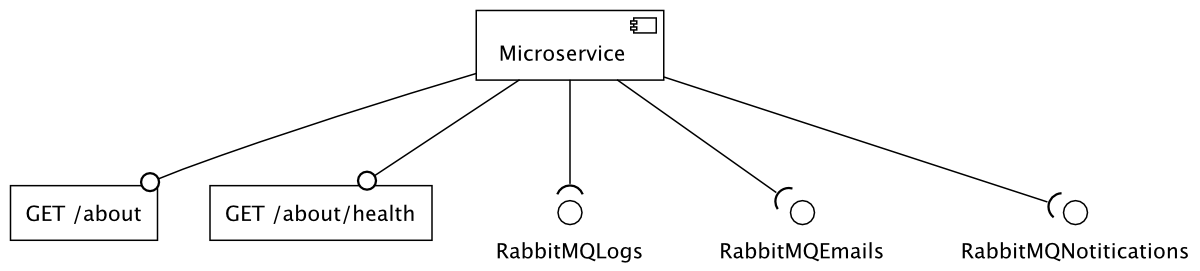
\includegraphics[max width=\textwidth]{assets/ms}
   \caption{Standardizované rozhraní mikroslužeb}\label{fig:ms-template}
\end{figure}

Kromě rozhraní šablona stanovuje základní konfigurace pro statickou analýzu kódu, sbírací a sestavovací nástroj, sdílené \h{.env} proměnné a další věci.
Nevýhodou však je, že se tato šablona musí manuálně udržovat a jakoukoliv změnu je nutné kopírovat do ostatních repozitářů.



\section{Správa dat a databáze}\label{sec:server-db}

Informační systém využívá pro uchovávání persistentních dat využívá dvou typů databází – \g{SQL} a NoSQL\@.
MongoDB, jakožto zástupce NoSQL databáze, byla zvolena pro uchovávání logů, jenž mají datovou složku, která vystupuje jako dynamická část dokumentu.
Vzhledem k pravděpodobnému budoucímu vyhledávání, případně indexaci části těchto dat, dané řešení je považováno za přiměřeně dobré.
Pro ukládání struktně strukturovaných dat, byla zvolena PostgreSQL databáze s uplatněným vzorem využití jedné databáze (schématu) pro každou mikroslužbu zvlášt.
Tuto volbu nejvíc ovlivnila potřeba tvorby další mikroslužby s migracemi, pokud by se použila jedna sdílená databáze.
Jak se zjistilo později, tak i největší problém takto rozdělených datových zdrojů – konzistence při transakčním zpracování – mohl být díky vhodné zvolené struktuře dat eliminován.

V důsledku takto zvoleného uspořádání každá mikroslužba se samostatně stará o data a strukturu vlastní části – v produkčním nasazení před spuštěním webového serveru kontroluje a případě aplikuje chybějící migrace, aniž by ovlivnila zbytek systému.
Jakéloiv přistupování k datům je rovněž komunikováno pouze přes mikroslužbu, ke které data patří.



\subsection{Správa projektů v git repozitářích}\label{subsec:server-db-github}

V původní realizaci \g{IS} správa projektů byla implementována jako systém se sadou dat v dokumentové databázi.
Z konceptuálního hlediska to bylo realtivině reacionální řešení – obsah projektu je \g{JSON} struktura, jež by se dala brát jako plnohodnotný dokument s dynamickou strukturou.
\g{CRUD} operace nad každou částí byly intuitivně prováděny, jistá nedokonalost však nastávala během odevzdávání iterace projektu.
V takovém případě bylo nutné vytvořit úplnou kopii všech částí projektu, aby se pro konkrétní odevzdání zachoval určitý stav.
To vedlo k celkem nepříjemnému problému zvětšování objemu databáze.

Z tohoto důvodu se vytvořil koncept ukládání obsahů projektů v samostatném git repozitáři, kde místo úplného kopírování částí projektu by se dala uchovávat postupná historie tvorby projektu.
Tím by se zamezilo zbytečné kopírování dat.

Se založením nového projektu v \g{IS} se tudíž zakládá i nový repozitář na Guthub, který byl zvolen kvůli poskytovanémi \g{API} jako git server (může být vyměněn za jakýkoliv jiný).
Párování mezi daty se základními informacemi o projektu (název apod.) a daty repozitáře se zajištuje s pomocí jednotného \g{UUID}, který je použit jako název repozitáře a zároveň uložen v databázi projektu.
Přístup k takovému repozitáři má pouze \g{IS}, nikoliv běžní uživatelé.

Vytvoření nové části obsahu projektu znamená vytvoření záznamu v relační databázi napárovaného na nově založený soubor v repozitáři.
Obsah souboru je postupně tvořen uživateli a ukládá datový \g{JSON} soubor, který je předáván z klientské části.
Aby nenastávaly konflikty v případě úpravy jedné části více uživateli je využíváno Github \g{API}, které pro každou aktualizaci souboru vyžaduje \h{md5} klíč předchozí verze souboru~\cite{githubupdate}.

Výše popsaná funkcionalita již byla realizována a ověřena z hlediska fungování.
Co se týče zbývající funkcionality – odevzdávání zafixovaného stacu částí projektu – tak by se mohla řešit s pomocí git značek (\h{tag}).
Jelikož úpravy projektu představují lineární historii, tak během přípravy náhledu odevzdáváného stavu by se samostné odevzdávání mohlo vázat ne na git větev, ale na určitý \h{hash}.
Takové odevzdání iterace by v tom případě znamenalo kromě vytvoření záznamu v databázi také tvorbu git značky, opět napárovaného na záznam dle \g{UUID}.
Pro zobrazení obsahu by se pak využívalo stahování dat částí z repozitáře v určitém historickém stavu.
